\documentclass{unswmaths}
\usepackage{unswshortcuts}
\usepackage{hyperref}
\usepackage{ dsfont }
\begin{document}
\author{Adam J. Gray}
\title{Assignment 3}
\subject{Ergodic Theory}
\studentno{3329798}

\unswtitle

\section{}
    We consider the map
    \begin{align}
        T(x) = 
        \begin{cases}
            2x + \frac{1}{2} & 0 \leq x < \frac{1}{4} \\
            -x + \frac{5}{4} & \frac{1}{4} \leq x < \frac{1}{2} \\
            -2x + \frac{7}{4} & \frac{1}{2} \leq x < \frac{3}{4} \\
            -x + 1 & \frac{3}{4} \leq x \leq 1.
        \end{cases}
    \end{align}
    This has the following plot:
    
    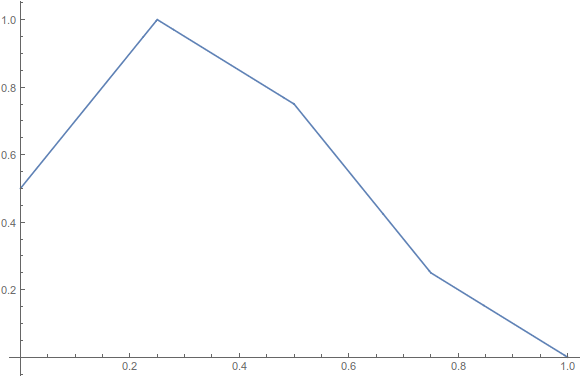
\includegraphics[scale=0.5]{qn_1_map}
\subsection{}
    We have that in general
    \begin{align}
        \mathcal{P}_T f(x) = \sum_{z \in T^{-1} x} \frac{f(z)}{|T'(z)|}.
    \end{align}
    Then in general we have
    \begin{align}
        T'(x) = 
        \begin{cases}
            2 & 0 \leq x < \frac{1}{4} \\
            -1 & \frac{1}{4} \leq x < \frac{1}{2} \\
            -2 & \frac{1}{2} \leq x < \frac{3}{4} \\
            -1 & \frac{3}{4} \leq x \leq 1.
        \end{cases}    
    \end{align}
    Also we can also see that
    \begin{align}
        T^{-1}\{x\} =
        \begin{cases}
            \{1-x\} & 0 \leq x < \frac{1}{4} \\
            \{\frac{7}{8} - \frac{x}{2} \} & \frac{1}{4} \leq x < \frac{1}{2} \\
            \{\frac{7}{8} - \frac{x}{2} \} \cup \{\frac{x}{2} - \frac{1}{4}\} & \frac{1}{2} \leq x < \frac{3}{4} \\
            \{\frac{5}{4} - x\} \cup \{ \frac{x}{2} - \frac{1}{4} \} & \frac{3}{4} \leq x < 1
        \end{cases}
    \end{align}
    thus for $ f_i(x) = \mathds{1}_{I_i}(x) $
    we have that
    \begin{align}
        \mathcal{P}_T f_1(x) &= \frac{1}{2}\mathds{1}_{I_3 \cup I_4}(x) = \frac{1}{2}\mathds{1}_{I_3}(x) + \frac{1}{2}\mathds{1}_{I_4}(x)\\
        \mathcal{P}_T f_2(x) &= \mathds{1}_{I_4}(x) \\
        \mathcal{P}_T f_3(x) &= \frac{1}{2}\mathds{1}_{I_2 \cup I_3}(x) = \frac{1}{2}\mathds{1}_{I_2}(x) + \frac{1}{2}\mathds{1}_{I_3}(x)\\
        \mathcal{P}_T f_4(x) &= \mathds{1}_{I_1}(x)
    \end{align}
\subsection{}
    Let $ \mathcal{S} = \operatorname{span} \bigcup_{i=1}^4 \mathds{1}_{I_i}$.
    
    Let $ f \in \mathcal{S} $ then $ f = \sum_{i=1}^4 \lambda_4 \mathds{1}_{I_i} $ and so by linearity of the Perron-Frobenius operator, we have that $ \mathcal{P}_T(f) = \sum_{i=1}^4 \lambda_4 \mathcal{P}_T(\mathds{1}_{I_i}) $ but from the result above we see that $ \mathcal{P}_T(\mathds{1}_{I_i}) \in \mathcal{S} $ for each $ i $ and so $ \mathcal{P} $ preserves $ \mathcal{S} $
\subsection{}
    We do this by just pluging the basis of $ \mathcal{S} $ into the $ \mathcal{P}_T $ and putting the results in each row of the matrix. Seeing as we already have first part we can just write down the matrix $ M $ as
    \begin{align}
        M = \left[ 
        \begin{array}{cccc}
            0 & 0 & \frac{1}{2} & \frac{1}{2} \\
            0 & 0 & 0 & 1 \\
            0 & \frac{1}{2} & \frac{1}{2} & 0 \\
            1 & 0 & 0 & 0 
        \end{array}
        \right]
    \end{align}
\subsection{}
    Using Mathematica we can calculate the left eigenvector corresponding to eigenvalue 1 which is
    \begin{align}
        \mathbf{v} = (1,\frac{1}{2},1,1)
    \end{align}
    which corresponds to the ACIM
    \begin{align}
        \mathds{1}_{I_1} + \frac{1}{2}\mathds{1}_{I_2} + \mathds{1}_{I_3} + \mathds{1}_{I_4}
    \end{align}
    
\section{}
\end{document}
